\chapter{T7 - Novo aprimoramento de uma Simulação: Laboratório e Experimento virus\_on\_network - Parte 2, por Isaque Augusto da Silva Santos (seraphritt)\label{desenho:experimento:jhcf}}

\section{Introdução}

Este capítulo apresenta a construção e uso do laboratório de simulações virus\_on\_network para a realização de experimentos que tem por objetivo investigar a hipótese causal letalidade-mortalidade que relaciona variáveis independentes e variáveis dependentes, supostamente presente nos estudos bibliométricos por mim.

É composto por mais cinco seções: 
\begin{enumerate}
    \item Descrição do fenômeno real;
    \item Apresentação do laboratório de simulações;
    \item Apresentação de análises exploratórias dos dados de experimentos realizados com o uso do laboratório;
    \item Discussão sobre \textit{insights} obtidos após os experimentos; e
    \item Conclusões.
\end{enumerate}

\section{O Fenômeno do Mundo Real}

O fenômeno do experimento em questão é a infecção por vírus e seu contágio ao haver contato entre pessoas. Esse é um acontecimento corriqueiro que está presente em qualquer sociedade na qual seres humanos compartilham o mesmo espaço físico \cite{delikhoon_modes_2021-1}, \cite{leung_transmissibility_2021}. 

Como pode-se ver na imagem \ref{fig:seraphritt:MinSaude} a seguir, esse fenômeno de contágio pode ocorrer de múltiplas formas.

\begin{figure}[H]
    \centering
    
\includegraphics[angle=0,width=1\textwidth]{exploratory-data-analysis/seraphritt/PesqBibliogr/Virus-Network/ESI4oudXkAAFOZk.jpg}
    \caption{Publicidade do Ministério da Saúde sobre o contágio do Coronavírus}
    \label{fig:seraphritt:MinSaude}
\end{figure}

As pessoas são os multiagentes e o contato entre elas é representado pelas arestas do grafo.

\section{O Laboratório virus\_on\_network}

O laboratório virus\_on\_network é um modelo genérico que simula a transmissão de um vírus em uma rede e pode ser utilizado tanto para simular uma infecção viral como uma infecção por um vírus em uma rede de computadores, como pode ser visto na descrição original do modelo \cite{f_stonedahl_netlogo_2008}.

Nesse ínterim, levando em conta o momento atual de preocupação com a prevenção de doenças virais como a Covid-19, escolhi usar esse modelo para simular uma epidemia. 

\subsection{O Conceito da Simulação}

O código base utilizado está presente no repositório do \textit{GitHub} denominado \textit{projectmesa/mesa-examples/Virus\_on\_network} \href{https://github.com/projectmesa/mesa-examples/tree/main/examples/Virus_on_Network}{link para o repositório}.

A arquitetura do modelo consiste em representar cada ser humano como um agente, criando assim uma rede de na qual os agentes se conectam. Portanto, as pessoas são os vértices e o contato entre elas é representado pelas arestas do grafo. Isso posto, existem quatro variáveis dependentes e oito variáveis independentes nesse modelo que serão especificadas posteriormente.

A simulação cria um ambiente que retrata o espalhamento de um vírus em uma sociedade. Por meio dessa simulação é possível notar relações entre as variáveis independentes e a alteração dos valores das variáveis dependentes, podendo significar uma relação de causa-efeito.

Os fenômenos que possivelmente podem estar relacionados com uma maior transmissão como, por exemplo,  a concentração populacional (quantidade de vértices), o frequência de contato (quantidade de arestas) entre as pessoas, chance de contágio do vírus (variável virus\_spread\_chance), chance de recuperação após infecção (variável recovery\_chance) e chance de letalidade (variável virus\_letal\_chance) foram explorados durante a simulação.

\subsection{O Simulador}

No código estão presentes as seguintes variáveis:
\begin{description}
\item \textit{virus\_letal\_chance} representa a chance de um vírus fazer com que o agente mude seu estado para morto (\textit{dead}).
\item \textit{num\_nodes} contém o número de agentes presentes no modelo.
\item \textit{avg\_node\_degree} representa o número médio de arestas entre os agentes, ou seja, o número médio de pessoas que podem estar infectadas caso um agente tenho o estado de \textit{infected}.
\item \textit{initial\_outbreak\_size} define a quantidade de agentes que iniciam com o estado de \textit{infected}.
\item \textit{virus\_spread\_chance} estipula a possibilidade de contágio do vírus.
\item \textit{virus\_check\_frequency} define a possibilidade de mudar o estado de um agente (\textit{infected} ou \textit{dead}).
\item \textit{recovery\_chance} representa a chance de um agente com o estado \textit{infected} mudar seu estado para \textit{suscetible}.
\item \textit{gain\_resistance\_chance} contém a chance de um agente mudar seu estado para \textit{resistant}.
\item \textit{stable} contém o valor que define se a simulação está estável ou não. Se o valor dessa variável for 0 significa que não está estável (False), se for 1 significa estabilidade da simulação (True). A condição de estabilidade definida foi: se houver 0 agentes com estado
\textit{Infected}, a simulação será considerada estável.
\end{description}

A seguinte imagem \ref{fig:seraphritt:interface} mostra interface gráfica do modelo:
\begin{figure}[H]
    \centering
    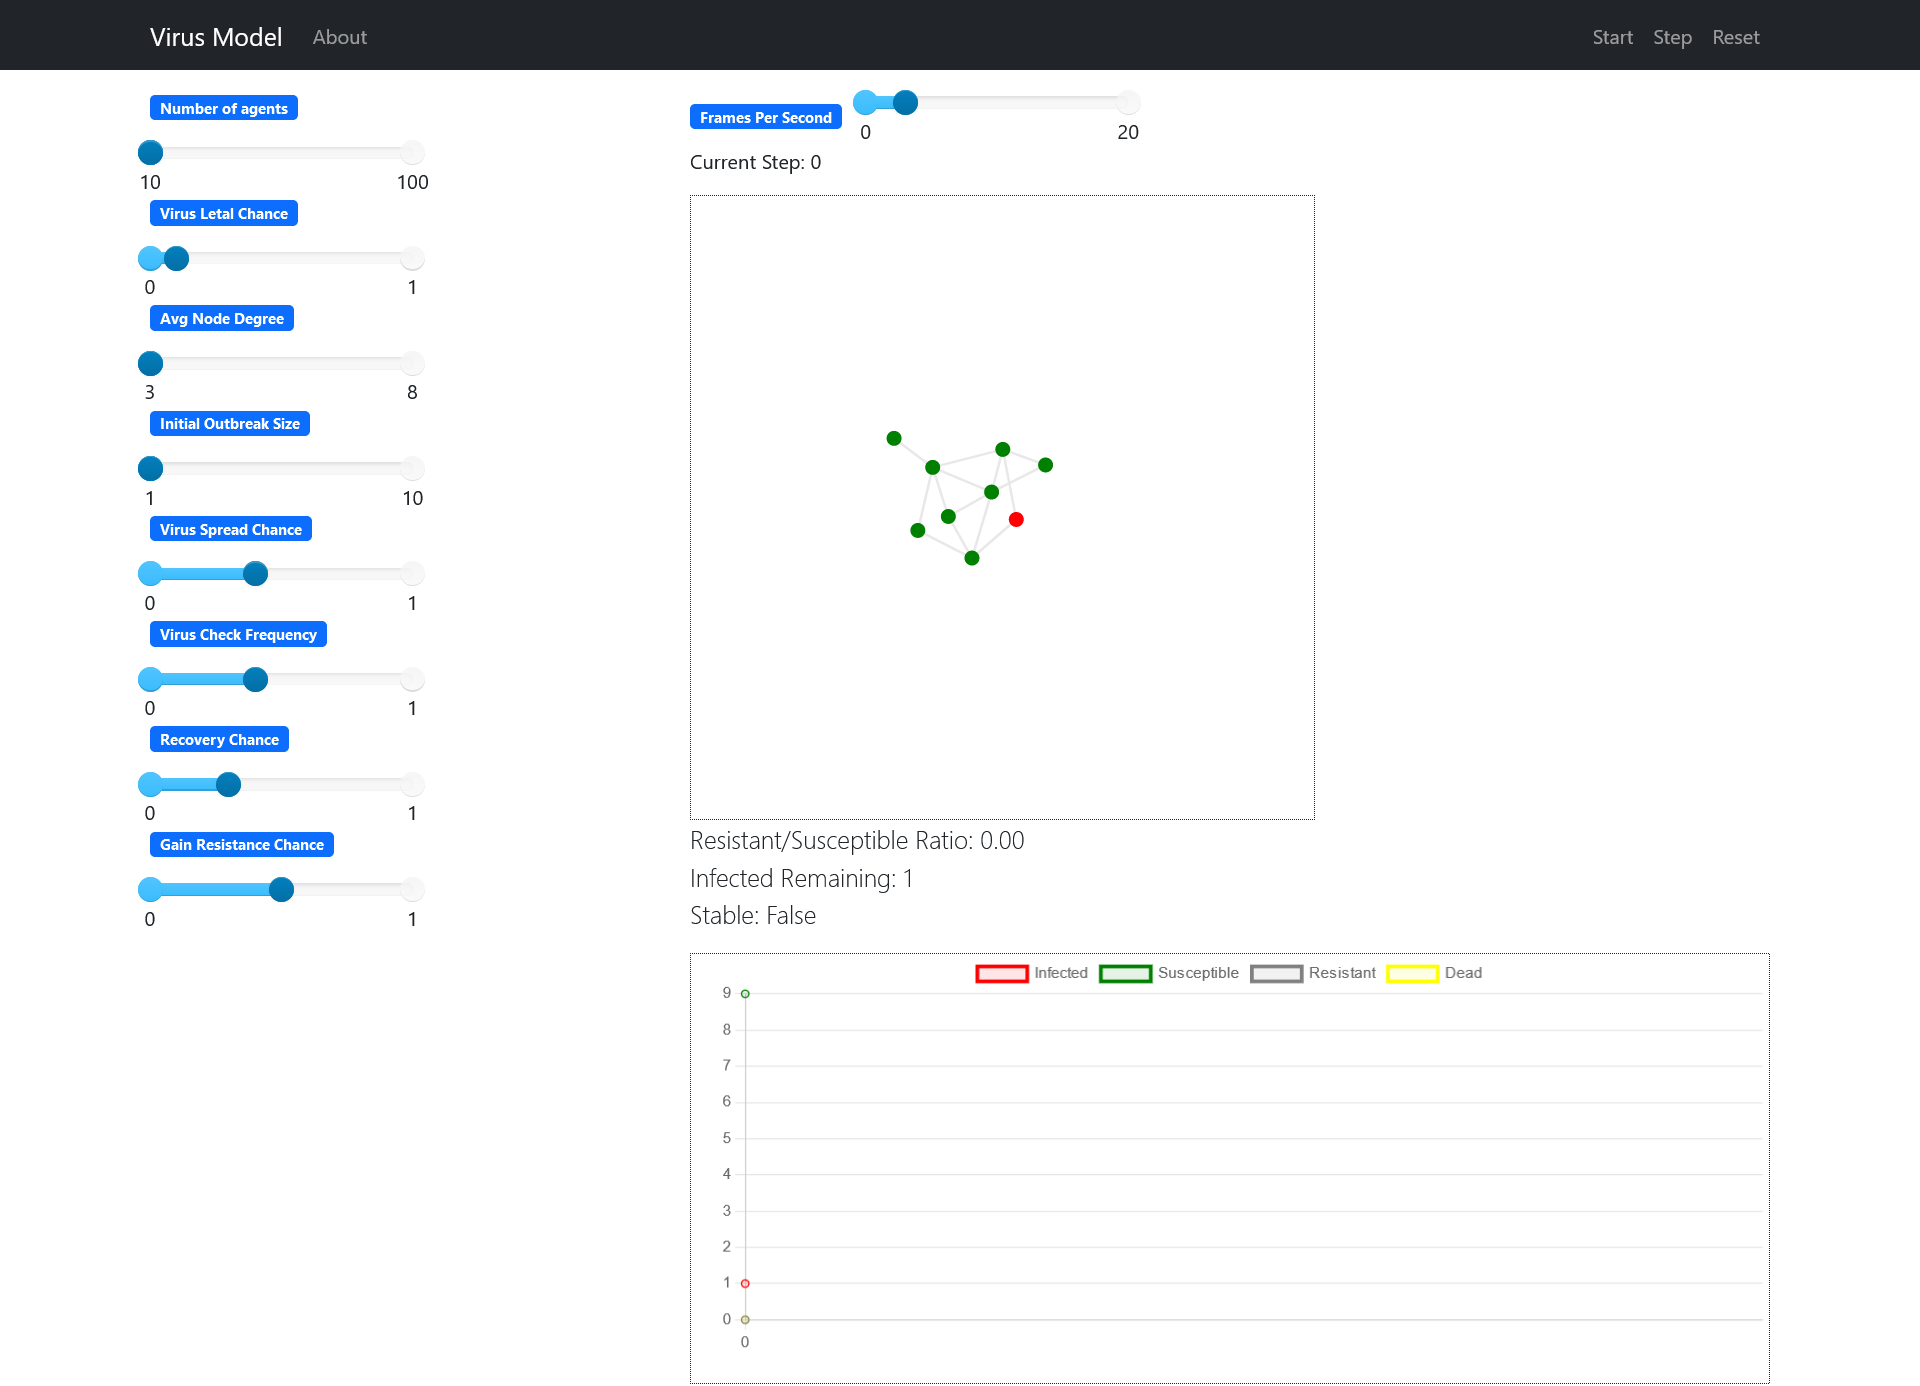
\includegraphics[angle=0,width=1\textwidth]{exploratory-data-analysis/seraphritt/PesqBibliogr/Virus-Network/Screenshot 2023-01-20 at 13-28-40 Virus Model (Mesa visualization).png}
    \caption{Interface gráfica do modelo}
    \label{fig:seraphritt:interface}
\end{figure}

\subsubsection{Variáveis Independentes ou de Controle}

São as seguintes as variáveis Independentes ou de Controle, manipuláveis na interface gráfica do simulador:
\begin{description}
\item Number of agents define a quantidade de agentes na simulação, ou seja, o quantidade de vértices no grafo, em um intervalo de 10 a 100.
\item Virus Letal Chance define a probabilidade do vírus mudar a cor do agente de vermelho (\textit{infected}) para amarelo (\textit{dead}), em um intervalo de 0 a 1.
\item Avg Node Degree é a quantidade média de arestas que cada vértice possui, em um intervalo de 3 a 8.
\item Initial Outbreak Size controla a quantidade de agentes na cor vermelha (\textit{infected} no primeiro passo da simulação, em um intervalo de 1 a 10.
\item Virus Spread Chance define a probabilidade dos vizinhos de um agente com a cor vermelha fazer com que seus vizinhos também fiquem com a cor vermelha, ou seja, infectados, em um intervalo de 0 a 1.
\item Virus Check Frequency controla a probabilidade da simulação mudar o estado de um agente para \textit{infected} ou \text{dead}, em um intervalo de 0 a 1.
\item Recovery Chance define a probabilidade de um agente ter sua cor mudada para verde (\textit{suscetible}) dado que está com a cor vermelha (\textit{infected}), em um intervalo de 0 a 1.
\item Gain Resistance Chance controla a probabilidade de um agente ter sua cor mudada para cinza (\textit{resistant}), em um intervalo de 0 a 1.
\end{description}

\subsubsection{Variáveis Dependentes}

São as seguintes as variáveis Dependentes, cujos valores são coletados e apresentados na interface gráfica do simulador:
\begin{description}
\item Infected apresenta a quantidade de agentes infectados.
\item Suscetible apresenta a quantidade de agentes suscetíveis a serem infectados. 
\item Resistant apresenta a quantidade de agentes resistentes ao vírus, ou seja, mesma que tenham contato com um agente infectado, esses agentes resistentes não serão infectados.
\item Dead apresenta a quantidade de agentes mortos. Esses agentes não trasmitem o vírus.
\item Stable representa a estabilidade do modelo.
\end{description}


\subsection{A Hipótese Causal}

A minha hipótese causal surgiu de questionamentos sobre a relação entre a letalidade e a transmissão de um vírus

\begin{description}
\item Será que um vírus com alta chance de letalidade consegue infectar uma grande quantidade de pessoas? 
\item Vírus com menor chance de letalidade necessariamente infectam um número maior de pessoas quando comparado a vírus extremamente letais?
\end{description}

Ademais, chegou-se a seguinte hipótese causal : ``A letalidade de um vírus não é a única variável independente responsável por uma grande quantidade de mortes por causa viral.``. 
Observação: Considera-se ``grande quantidade`` um número próximo ou igual a quantidade de agentes suscetíveis à infecção viral.

A hipótese causal foi obtida com o auxílio dos artigos \cite{geoghegan_virological_2016} e \cite{belay_low-incidence_2014}.

%Apresentar a hipótese causal modelada com o uso da ferramenta Loopy.

%Apresentar, de forma gráfica, exemplos de execução da hipótese causal, na ferramenta Loopy.

% \begin{figure}
%     \centering
%     \includegraphics[width=0.5\textwidth]{experiments/jhcf/ExperimentoProducaoCiencia/Causal.png}
%     \caption{Modelo causal de simulação XYZ. Para ver o modelo visite  \url{https://bit.ly/3qDmXwj}.}
%     \label{fig:jhcf:EXP:xyz:modelo:causal}
% \end{figure}

% \begin{figure}
%     \centering
%     \includegraphics[width=0.5\textwidth]{experiments/jhcf/ExperimentoProducaoCiencia/Simulacao.png}
%     \caption{Simulação do modelo causal de simulação XYZ. }
%     \label{fig:jhcf:EXP:xyz:simulacao:modelo:causal}
% \end{figure}

% Prover uma url (usar o bit.ly, conforme indica a interface gráfica do Loopy, na opção ``Save as link'') para que o leitor possa ele mesmo executar a simulação no Loopy.

\subsection{O Código do Simulador}

Com o intuito de comprovar a veracidade da hipótese causal, adicionei uma variável independente \textit{Virus Letal Chance} e uma variável dependente \text{Dead} para aprimorar o modelo e assim simular a infecção por vírus com chances de letalidade diferentes. 

As classes presentes no simulador são:
\begin{description}
    \item \textit{State}, classe responsável por controlar o estado de cada agente e possui os atributos \textit{SUSCETIBLE = 0}, \textit{INFECTED = 1}, \textit{RESISTANT = 2} e \textit{DEAD = 3}.
    \item \textit{VirusAgent}, classe resposável por declarar os agentes.
    \item \textit{VirusOnNetwork}, classe resposável pelo modelo em si, bem como a coleta de dados. Essa classe instancia os agentes. 
\end{description}

A criação e o modelo de agentes pode ser vista no trecho de código a seguir:

\begin{verbatim}
class VirusOnNetwork(mesa.Model):
    """A virus model with some number of agents"""

    def __init__(
        self,
        virus_letal_chance=0.1, #mod
        num_nodes=10,
        avg_node_degree=3,
        initial_outbreak_size=1,
        virus_spread_chance=0.4,
        virus_check_frequency=0.4,
        recovery_chance=0.3,
        gain_resistance_chance=0.5,
    ):
        self.virus_letal_chance = virus_letal_chance
        self.num_nodes = num_nodes
        prob = avg_node_degree / self.num_nodes
        self.G = nx.erdos_renyi_graph(n=self.num_nodes, p=prob)
        self.grid = mesa.space.NetworkGrid(self.G)
        self.schedule = mesa.time.RandomActivation(self)
        self.initial_outbreak_size = (
            initial_outbreak_size if initial_outbreak_size <= num_nodes else num_nodes
        )
        self.virus_spread_chance = virus_spread_chance
        self.virus_check_frequency = virus_check_frequency
        self.recovery_chance = recovery_chance
        self.gain_resistance_chance = gain_resistance_chance

        self.datacollector = mesa.DataCollector(
            {
                "Infected": number_infected,
                "Susceptible": number_susceptible,
                "Resistant": number_resistant,
                "Dead": number_dead,
            }
        )

        # Create agents
        for i, node in enumerate(self.G.nodes()):
            a = VirusAgent(
                i,
                self,
                State.SUSCEPTIBLE,
                self.virus_spread_chance,
                self.virus_check_frequency,
                self.recovery_chance,
                self.gain_resistance_chance,
                self.virus_letal_chance,
            )
            self.schedule.add(a)
            # Add the agent to the node
            self.grid.place_agent(a, node)

        # Infect some nodes
        infected_nodes = self.random.sample(list(self.G), self.initial_outbreak_size)
        for a in self.grid.get_cell_list_contents(infected_nodes):
            a.state = State.INFECTED

        self.running = True
        self.datacollector.collect(self)

    def resistant_susceptible_ratio(self):
        try:
            return number_state(self, State.RESISTANT) / number_state(
                self, State.SUSCEPTIBLE
            )
        except ZeroDivisionError:
            return math.inf

    def step(self):
        self.schedule.step()
        # collect data
        self.datacollector.collect(self)

    def run_model(self, n):
        for i in range(n):
            self.step()


class VirusAgent(mesa.Agent):
    def __init__(
        self,
        unique_id,
        model,
        initial_state,
        virus_spread_chance,
        virus_check_frequency,
        recovery_chance,
        gain_resistance_chance,
        virus_letal_chance,
    ):
        super().__init__(unique_id, model)

        self.state = initial_state

        self.virus_spread_chance = virus_spread_chance
        self.virus_check_frequency = virus_check_frequency
        self.recovery_chance = recovery_chance
        self.gain_resistance_chance = gain_resistance_chance
        self.virus_letal_chance = virus_letal_chance

    def try_to_infect_neighbors(self):
        neighbors_nodes = self.model.grid.get_neighbors(self.pos, include_center=False)
        susceptible_neighbors = [
            agent
            for agent in self.model.grid.get_cell_list_contents(neighbors_nodes)
            if agent.state is State.SUSCEPTIBLE
        ]
        for a in susceptible_neighbors:
            if self.random.random() < self.virus_spread_chance and a.state is not State.DEAD:
                a.state = State.INFECTED

    def try_gain_resistance(self):
        if self.random.random() < self.gain_resistance_chance:
            self.state = State.RESISTANT

    def try_remove_infection(self):
        # Try to remove
        if self.random.random() < self.recovery_chance:
            # Success
            self.state = State.SUSCEPTIBLE
            self.try_gain_resistance()
        else:
            # Failed
            self.state = State.INFECTED

    def try_check_situation(self):
        if self.random.random() < self.virus_check_frequency:
            # Checking...
            if self.state is State.INFECTED:
                self.try_remove_infection()
            if self.state is State.INFECTED and self.random.random() < self.virus_letal_chance: # if infection is not removed and
            # letal chance of the virus is enough, agent is considered dead
            # dead agents cannot transmit the virus
                self.state = State.DEAD

    def step(self):
        if self.state is State.INFECTED:
            self.try_to_infect_neighbors()
        self.try_check_situation()
\end{verbatim}

O comportamento do modelo e dos agentes a cada passo pode ser visto nos seguintes trechos de código:

\begin{verbatim}
def number_state(model, state):
    return sum(1 for a in model.grid.get_all_cell_contents() if a.state is state)


def number_infected(model):
    return number_state(model, State.INFECTED)


def number_susceptible(model):
    return number_state(model, State.SUSCEPTIBLE)


def number_resistant(model):
    return number_state(model, State.RESISTANT)

def number_dead(model): #mod
    return number_state(model, State.DEAD)

\end{verbatim}

\begin{verbatim}
 def step(self):
        self.schedule.step()
        # collect data
        self.datacollector.collect(self)

    def run_model(self, n):
        for i in range(n):
            self.step()
\end{verbatim}

\begin{verbatim}
def try_to_infect_neighbors(self):
        neighbors_nodes = self.model.grid.get_neighbors(self.pos, include_center=False)
        susceptible_neighbors = [
            agent
            for agent in self.model.grid.get_cell_list_contents(neighbors_nodes)
            if agent.state is State.SUSCEPTIBLE
        ]
        for a in susceptible_neighbors:
            if self.random.random() < self.virus_spread_chance and a.state is not State.DEAD:
                a.state = State.INFECTED

    def try_gain_resistance(self):
        if self.random.random() < self.gain_resistance_chance:
            self.state = State.RESISTANT

    def try_remove_infection(self):
        # Try to remove
        if self.random.random() < self.recovery_chance:
            # Success
            self.state = State.SUSCEPTIBLE
            self.try_gain_resistance()
        else:
            # Failed
            self.state = State.INFECTED

    def try_check_situation(self):
        if self.random.random() < self.virus_check_frequency:
            # Checking...
            if self.state is State.INFECTED:
                self.try_remove_infection()
            if self.state is State.INFECTED and self.random.random() < self.virus_letal_chance: # if infection is not removed and
            # letal chance of the virus is enough, agent is considered dead
            # dead agents cannot transmit the virus
                self.state = State.DEAD

    def step(self):
        if self.state is State.INFECTED:
            self.try_to_infect_neighbors()
        self.try_check_situation()
\end{verbatim}



% \lstinputlisting[numbers=left,language={Python},basicstyle=\tiny\ttfamily,caption={Código da Criação de um agente.},label={code:jhcf:EXP:xyz:batch:run},firstnumber=110,firstline=110,lastline=127]
% {labs/jhcf/ExperimentoProducaoCiencia/model.py}


%Observe que a descrição do simulador batch deve ser suficientemente detalhada para evidenciar o desenho do experimento, a seleção e (ou) coleta de valores das variáveis independentes, de controle e dependentes.

\section{Os Experimentos Realizados}

Foram feitos 2 experimentos principais para verificar a veracidade da hipótese causal:
\begin{description}
\item Experimento 1 com a variável \textit{Virus Letal Chance} com o valor máximo e as outras variáveis com um valor aleatório. Esse experimento tem como objetivo verificar se a variável \textit{Virus Letal Chance} é dominante sobre as outras variáveis e por si só faz com que a quantidade de mortes aumente significativamente.
\item Experimento 2 com a variável \textit{Virus Letal Chance} com o valor máximo e \textit{Virus Spread Chance} com valor máximo e \textit{Recovery Chance} com valor mínimo, com o intuito de achar alguma configuração de variáveis na qual o número de mortes seja ampliado significativamente. 
\end{description}
Além desses 2 experimentos principais, foram feitos diversos outros experimentos modificando o valor de todas as variáveis para encontrar outras configurações que fariam com que o número de mortes fosse o mínimo ou o máximo.

Devido a quantidade de variáveis, houve uma certa dificuldade em achar relações de causa e efeito de uma variável independente isolada com uma variável dependente. Isso deve-se ao fato da complexidade do fenômeno de infecção viral.

Ademais, notou-se a necessidade de simplificar o modelo, tendo em vista também essa complexidade dita anteriormente. Isso posto, variáveis como a chance de mutabilidade do vírus e de reinfecção, por exemplo, não foram adicionadas. 

A imagem \ref{fig:seraphritt:Graf} a seguir apresenta o gráfico obtido após o experimento 1.

\begin{figure}[H]
    \centering
    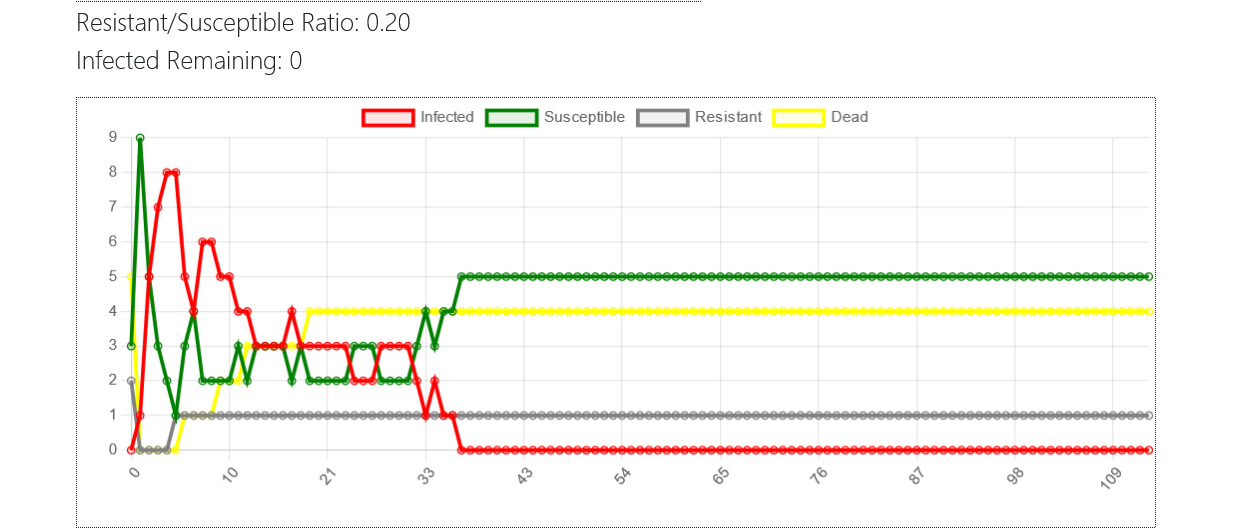
\includegraphics[angle=0,width=1\textwidth]{exploratory-data-analysis/seraphritt/PesqBibliogr/Virus-Network/grafico_compexp.png}
    \caption{Gráfico obtido no experimento 1}
    \label{fig:seraphritt:Graf}
\end{figure}

Adicionou-se também um novo arquivo com o nome \textit{experimentos\_estatisticos.py}, com o intuito de auxiliar na coleta dos dados das simulações, como pode ser visto na próxima seção.
\subsection{Os Dados Coletados}

A coleta dos dados das simulações foram feitas seguindo uma sequência de critérios para facilitar as conclusões sobre os dados encontrado. Esses critérios foram:
 \begin{description}
\item\textit As variáveis independentes \textit{Number of agents}, \textit{Avg Node Degree}, \textit{Initial Outbreak Size}, \textit{Virus Spread Chance}, \textit{Virus Check Frequency}, \textit{Recovery Chance} e \textit{Gain Resistance Chance}
tiveram seus valores definidos como constantes, ou seja, durante a série de experimentos feitos para coleta de dados  o valor dessas variáveis não muda.
\item  \textit{Number of agents} com valor constante de 10.
\item  \textit{Avg Node Degree} com valor constante de 3.
\item \textit{Initial Outbreak Size} com valor constante de 1.
\item  \textit{Virus Spread Chance} com valor constante de 0,4.
\item \textit{Virus Check Frequency} com valor constante de 0,4.
\item  \textit{Recovery Chance} com valor constante de 0,3.
\item \textit{Gain Resistance Chance} com valor constante de 0,5.
\item \textit Foram feitos experimentos com números de replicações diferentes para obter maior grau de certeza. Portanto, houve experimentos com 50, 100, 200 e 400 replicações.
\item \textit Como a hipótese causal refere-se á letalidade e sua singularidade no aumento do número de mortes, somente a variável \textit{Virus Letal Chance} deve seu valor modificado entre os experimentos, com um intervalo de 0.1, indo de 0 (valor mínimo) até 1 (valor máximo.
\end{description}

Variáveis presentes nos histogramas:
\begin{description}
\item\textit{ Frequency}: O número de ocorrências de determinado 
\item \textit{Dead Agents} O número de agentes com o estado \textit{Dead}.
\end{description}

O primeiro histograma \ref{fig:seraphritt:hist1} foi feito com 50 replicações e é possível notar a grande concentração de ocorrências de 0 agentes com estado \textit{Dead}, ou seja, a quantidade mínima de agentes.
Semelhantemente, nota-se o mesmo resultado com o número de replicações igual a 100 \ref{fig:seraphritt:hist2}, 200 \ref{fig:seraphritt:hist3} e 400 \ref{fig:seraphritt:hist4}. Com isso pode-se concluir que a modificação da letalidade do vírus, por si só, não consegue aumentar significadamente o número de mortes, fazendo com que esse número seja próximo da quantidade máxima de agentes.  

\begin{figure}[H]
    \centering
    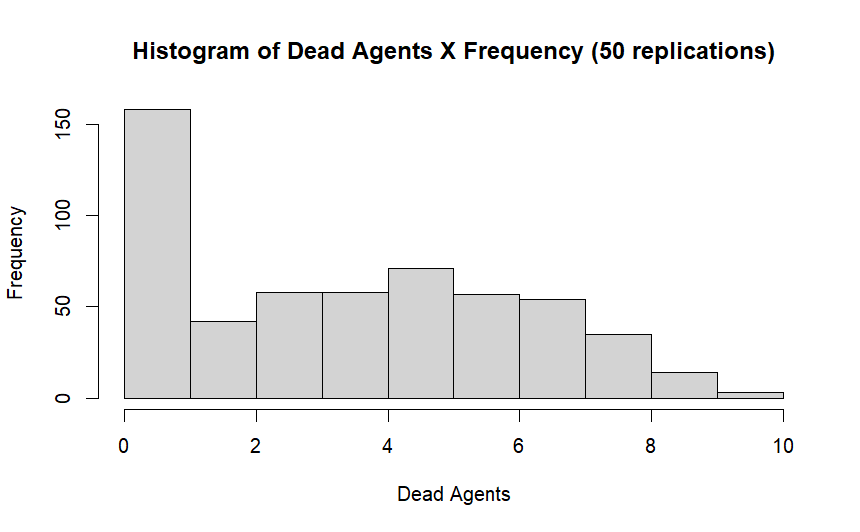
\includegraphics[angle=0,width=1\textwidth]{exploratory-data-analysis/seraphritt/PesqBibliogr/Virus-Network/Hist_50_repl.png}
    \caption{Histograma obtido a partir dos dados do experimento realizado com 50 replicações}
    \label{fig:seraphritt:hist1}
\end{figure}


\begin{figure}[H]
    \centering
    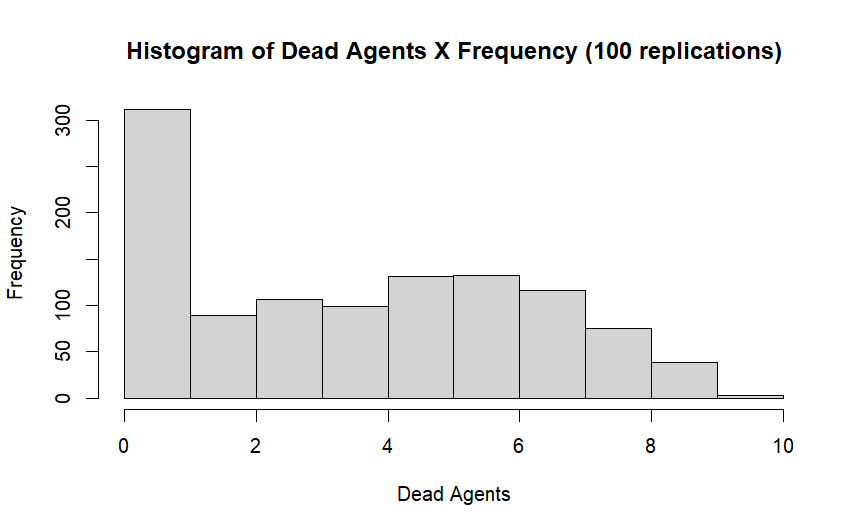
\includegraphics[angle=0,width=1\textwidth]{exploratory-data-analysis/seraphritt/PesqBibliogr/Virus-Network/Hist_100_repl.png}
    \caption{Histograma obtido a partir dos dados do experimento realizado com 100 replicações}
    \label{fig:seraphritt:hist2}
\end{figure}

\begin{figure}[H]
    \centering
    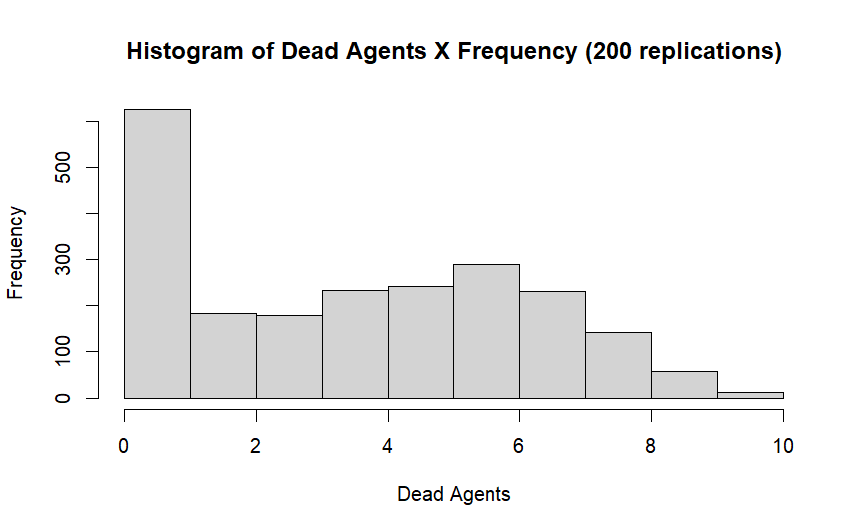
\includegraphics[angle=0,width=1\textwidth]{exploratory-data-analysis/seraphritt/PesqBibliogr/Virus-Network/Hist_200_repl.png}
    \caption{Histograma obtido a partir dos dados do experimento realizado com 200 replicações}
    \label{fig:seraphritt:hist3}
\end{figure}

\begin{figure}[H]
    \centering
    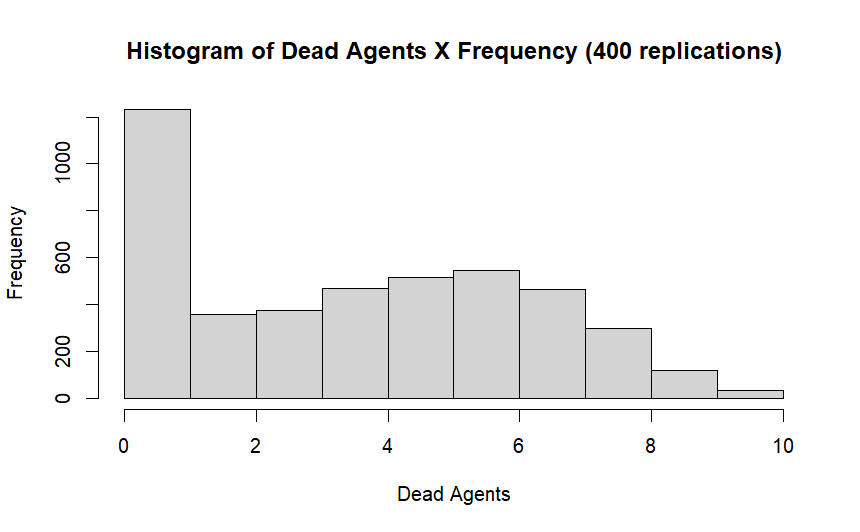
\includegraphics[angle=0,width=1\textwidth]{exploratory-data-analysis/seraphritt/PesqBibliogr/Virus-Network/Hist_400_repl.png}
    \caption{Histograma obtido a partir dos dados do experimento realizado com 400 replicações}
    \label{fig:seraphritt:hist4}
\end{figure}

Variáveis presentes nos\textit{boxplots}:
\begin{description}
\item\textit{Virus Lethal Chance}: A probabilidade de um agente com estado \textit{Infected} ter seu estado mudado para \textit{Dead}. 
\item \textit{Dead Agents} O número de agentes com o estado \textit{Dead}.
\end{description}

Os boxplots com 50 \ref{fig:seraphritt:bp1}, 100 \ref{fig:seraphritt:bp2}, 200 \ref{fig:seraphritt:bp3} e 400 \ref{fig:seraphritt:bp4} replicações também demonstram dados que concluem que a letalidade do vírus sozinha não maximiza a quantidade de mortes. Nota-se que mesmo com a letalidade em valores altos, como 70\%, 80\%, 90\% e até 100\%, os valores se concentram entre 4 e 5 agentes com estado \textit{Dead}. 

\begin{figure}[H]
    \centering
    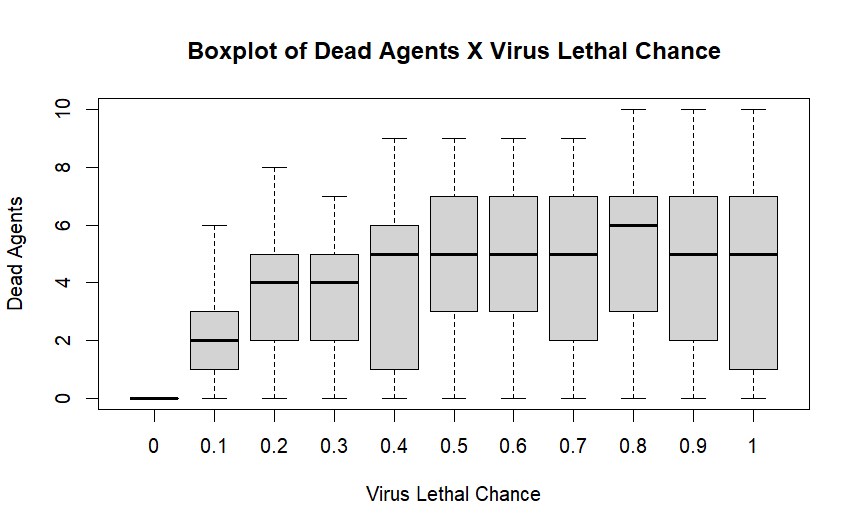
\includegraphics[angle=0,width=1\textwidth]{exploratory-data-analysis/seraphritt/PesqBibliogr/Virus-Network/Boxplot_50_repl.png}
    \caption{\textit{Boxplot} obtido a partir dos dados do experimento realizado com 50 replicações}
    \label{fig:seraphritt:bp1}
\end{figure}

\begin{figure}[H]
    \centering
    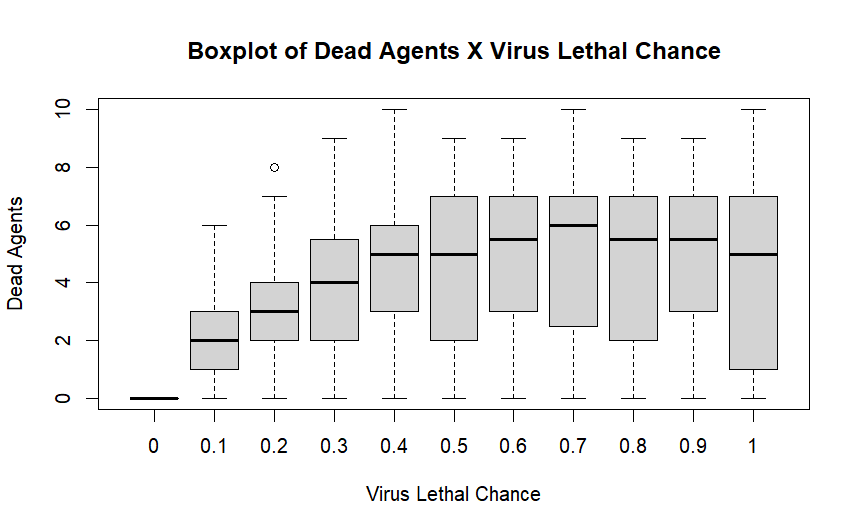
\includegraphics[angle=0,width=1\textwidth]{exploratory-data-analysis/seraphritt/PesqBibliogr/Virus-Network/Boxplot_100_repl.png}
    \caption{\textit{Boxplot} obtido a partir dos dados do experimento realizado com 100 replicações}
    \label{fig:seraphritt:bp2}
\end{figure}

\begin{figure}[H]
    \centering
    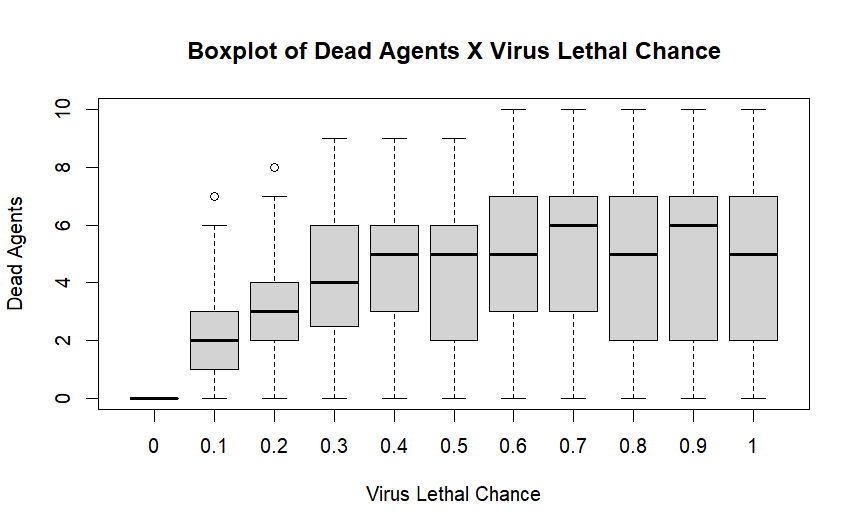
\includegraphics[angle=0,width=1\textwidth]{exploratory-data-analysis/seraphritt/PesqBibliogr/Virus-Network/Boxplot_200_repl.png}
    \caption{\textit{Boxplot} obtido a partir dos dados do experimento realizado com 200 replicações}
    \label{fig:seraphritt:bp3}
\end{figure}

\begin{figure}[H]
    \centering
    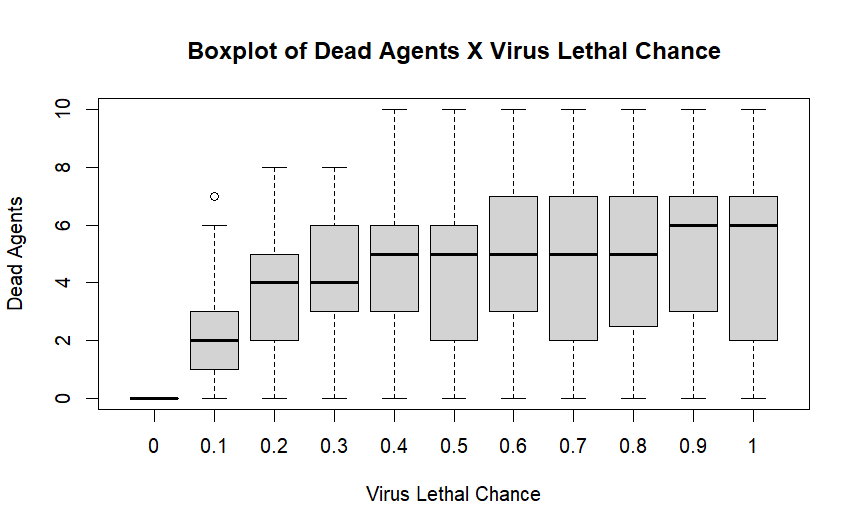
\includegraphics[angle=0,width=1\textwidth]{exploratory-data-analysis/seraphritt/PesqBibliogr/Virus-Network/Boxplot_400_repl.png}
    \caption{\textit{Boxplot} obtido a partir dos dados do experimento realizado com 400 replicações}
    \label{fig:seraphritt:bp4}
\end{figure}

A seguir pode-se ver uma parte de uma tabela \ref{tab:tabelareduz:1} (as tabelas completas possuem ao menos 220 linhas) usada para a geração dos histogramas e dos \textit{boxplots}.

Variáveis presentes na tabela:
\begin{description}
\item Virus Letal Chance:  A probabilidade de um agente com estado \textit{Infected} ter seu estado mudado para \textit{Dead}. 
\item Infected: Número de agentes com estado \textit{Infected}.
\item Suscetible: Número de agentes com estado \textit{Suscetible}.
\item Resistant: Número de agentes com estado \textit{Resistant}.
\item Dead: Número de agentes com estado \textit{Dead}.
\item Stable: Variável que define a estabilidade da simulação, sendo que 0 significa não estável e 1 significa estável.
\end{description}

\begin{table}[!ht]
    \centering
    \begin{tabular}{|l|l|l|l|l|l|}
    \hline
        virus\_letal\_chance & Infected & Susceptible & Resistant & Dead & Stable \\ \hline
        0.0 & 0 & 3 & 7 & 0 & 1 \\ \hline
        0.1 & 0 & 3 & 4 & 3 & 1 \\ \hline
        0.2 & 0 & 4 & 1 & 5 & 1 \\ \hline
        0.30000000000000004 & 0 & 3 & 3 & 4 & 1 \\ \hline
        0.4 & 0 & 0 & 3 & 7 & 1 \\ \hline
        0.5 & 0 & 1 & 2 & 7 & 1 \\ \hline
        0.6000000000000001 & 0 & 0 & 6 & 4 & 1 \\ \hline
        0.7000000000000001 & 0 & 1 & 4 & 5 & 1 \\ \hline
        0.8 & 0 & 1 & 2 & 7 & 1 \\ \hline
        0.9 & 0 & 0 & 0 & 10 & 1 \\ \hline
        1.0 & 0 & 9 & 0 & 1 & 1 \\ \hline
        0.0 & 0 & 1 & 9 & 0 & 1 \\ \hline
        0.1 & 0 & 3 & 5 & 2 & 1 \\ \hline
        0.2 & 0 & 1 & 4 & 5 & 1 \\ \hline
        0.30000000000000004 & 0 & 1 & 3 & 6 & 1 \\ \hline
        0.4 & 0 & 2 & 1 & 7 & 1 \\ \hline
        0.5 & 0 & 5 & 2 & 3 & 1 \\ \hline
        0.6000000000000001 & 0 & 0 & 2 & 8 & 1 \\ \hline
        0.7000000000000001 & 0 & 3 & 2 & 5 & 1 \\ \hline
    \end{tabular}
\caption{Tabela reduzida obtida a partir dos dados do experimento com 50 replicações}
\label{tab:tabelareduz:1} 
\end{table}

% Exemplificar alguns registros presentes em cada um dos arquivos, usando o comando csvreader. 
% Ver exemplo a seguir.


% \begin{table}[htp]
%     \centering
% \footnotesize
% \csvreader[
% separator=comma, % especifica o separador de colunas
% tabular = {|r|l|r|r|r|r|}, 
% filter={\value{csvrow}<20}, % indica quantas colunas devem ser apresentadas
% %,filter not strcmp={\csvcolii}{},
% table head = \hline\hline \# & Initial Trading \%	& Alpha & Beta & Available & Decease Rate\\ \hline\hline, % cabeçalho da tabela
% table foot = \hline\hline] % rodapé da tabela
% {experiments/jhcf/ExperimentoProducaoCiencia/data.csv} % arquivo de onde os dados devem ser lidos
% {InitialTradingPerc=\trading,AlphaAjuste=\salpha,BetaAjuste=\sbeta,Available=\avail,ChannelsDeceasedRate=\deceaserate} % mapeia os nomes das colunas no CSV para variáveis a serem usadas na linha de detalhe, abaixo
% { \thecsvrow & \trading & \salpha & \sbeta & \avail & \deceaserate} % valores a serem mostrados nas linhas
% \caption{Apresentando alguns  registros mantidos em um arquivo CSV.}
%     \label{tab:jhcf:EXP:xyz:registros:modelo}
% \end{table}

% \subsection{Análises exploratórias preliminares}

% Apresentar as distribuições de frequência dos valores obtidos para as variáveis dependentes, em função de cada configuração de valores para variáveis independentes.

% Plotar graficamente essas distribuições de frequência e discutir as variações observadas, em termos de média (ou moda) e desvio padrão. Constatar a normalidade ou não normalidade das distribuições de frequência, quando possível.

% Nas plotagens, usar o R Studio, com o comando hist(). Ao gerar as plotagens no R Studio, usar a opção ``Plots -> Export -> Save as PDF'', para que as imagens sejam geradas de forma vetorial, e não percam qualidade quando redimensionadas.


% \begin{figure}
%     \centering
%     \includegraphics[page=1,clip=true,trim={0 1cm 1.5cm 2cm},width=\textwidth,height=0.5\textheight]{experiments/jhcf/ExperimentoProducaoCiencia/Rplot02.pdf}
%     \caption{Distribuição de Frequência no número de nós infectados em 300 experimentos, após 100 passos de simulação em cada experimento, com numNodes==100, virusSpreadChance==0.9.}
%     \label{fig:jhcf:EXP:xyz:distfreq}
% \end{figure}



\section{Discussão e \textit{insights} preliminares sobre as hipóteses}

Considerando a simplificação do fenômeno modelado em comparação com o fenômeno real de infecção viral, nota-se que em vista dos resultados obtidos nos diversos experimentos, inicialmente comprova-se a hipótese causal. 

O experimento principal 1 prova que a letalidade por si só não consegue dominar sobre as outras variáveis e não causa um grande número de mortes. A exemplo, se a taxa de transmissão for baixa(com valores entre 0 e 0.1), mesmo a letalidade sendo máxima, o número de mortes não é suficientemente grande.

Ademais, o experimento principal 2 apresenta uma configuração de variáveis na qual o número de mortes é próximo ao máximo e essa configuração depende dos valores de 3 variáveis.

Com o auxílio dos dados coletados nesse experimento, pode-se reafirmar por meio dos histogramas e \textit{boxsplots} a comprovação da hipótese causal. 

\section{Conclusão}

Ao finalizar o experimento foi possível obter a resposta para os dois questionamentos que originaram a hipótese causal. Em relação a primeira pergunta, foi possível concluir que um vírus com alta letalidade pode infectar e consequentemente causar a morte de uma grande quantidade de pessoas se houver outras condições para isso, como por exemplo uma pequena taxa de resistência ao vírus e uma grande taxa de transmissão.

Já em relação a segunda pergunta, interpreta-se que não necessariamente existe essa relação de superioridade da quantidade de pessoas infectadas com um vírus menos letal, uma vez que foi achada uma configuração onde um vírus com letalidade máxima infectou um número bem próximo a quantidade de agentes. 

Entretanto, existem várias questões não respondidas devido a simplificação do modelo. Por exemplo, indagações como quais outras variáveis influenciam na infecção viral (mutabilidade do vírus, resistência a antivirais, etc.) ou como os métodos de isolamento e de higiene pessoal influem na quantidade de infectados.   